
\section{Accelerators and Detectors: the LHC and the CMS}
\label{sec:org3878a16}
\subsection{The Large Hadron Collider}
\label{sec:org5906b28}
Our knowledge in the field of high energy physics has been largely obtained through fixed target experiments that used proton and electron accelerators. However, over the last decades, the significance of colliding beam experiments has been rising. Such experiments involve two particle beams that rotate in opposite directions and collide at multiple points around the ring. The key advantage of colliding beam machines is their ability to produce new particles due to the high center of mass energy created during the collision. This energy increases linearly as E, rather than as \(E^{1/2}\), in fixed target experiments, and almost all of it is utilized in generating new particles[modern particle physics].

One great example of a colliding beam machine is The Large Hadron Collider (LHC).  The LHC has been instrumental in many groundbreaking discoveries, with the most famous one beeing the Higgs boson, and has helped scientists to further our understanding of the fundamental nature of the universe. The LHC encompasses a 27-kilometre ring consisting of superconducting magnets with numerous accelerating structures along its length.

Within the accelerator, a strong magnetic field is accelerating the two counterrotating proton beams to velocities near that of the speed of light uppon collision.  The thousands of  superconducting magnets, responsible of the generation of the magnetic field, are of varying sizes and types. Dipole magnets, 1232 in total and 15 meters in length, are utilized to bend the beams and quadrupole magnets, 392 in total and 5-7 meters long, focus the beams. Prior to collision, another type of magnet is used to compress the particles, increasing the likelihood of collisions \href{https://www.lhc-closer.es/taking\_a\_closer\_look\_at\_lhc/0.momentum}{source}.
\subsection{The Compact Muon Solenoid}
\label{sec:orgccfbfe1}
The main goal of  the Compact Muon Solenoid (CMS), as a general purpose particle detector, is to  to reconstruct the Feynman diagram associated with any interaction that might happen inside the LHC. The first and foremost interactions that happen are the collisions between the beams, which generate individual interactions known as \emph{events}. Even though most of the particles associated with an event are unstable, their final decay products, are stable enough to reach the detector and be measured. In the rest of the chapter I will give a brief overview of the CMS detector and discus how does it detect particles.
\subsubsection{Overview}
\label{sec:org3cfeb42}
The CMS detector consists of 5 compartments, each with unique functionality, that are organised in several coaxial layers. The Silicon Tracker, located in the innermost part of CMS, includes silicon pixel vertex detectors and silicon strip detectors, which trace the position and momentum of charged particles. The Electromagnetic Calorimeter (ECAL), the second layer, is composed of PbWO4 crystals and intended to detect photons and electrons. The Hadronic Calorimeter (HCAL), the third layer, is designed to identify hadrons. The Superconducting Solenoid Magnet, the fourth layer, is an solenoid coil that generates a constant magnetic field of 4 T along the direction of the  beam. Due to the deflection of the trajectories of charged particles by the magnet, it becomes possible to measure their momentum. The final, outer most layer, is responsible for the measurement of muon the tracks. Figure \ref{fig:CMS_detector} provides a sectional view of the CMS detector[\url{https://cms.cern/news/cms-detector-design}].
\begin{figure}[hb]
\centering
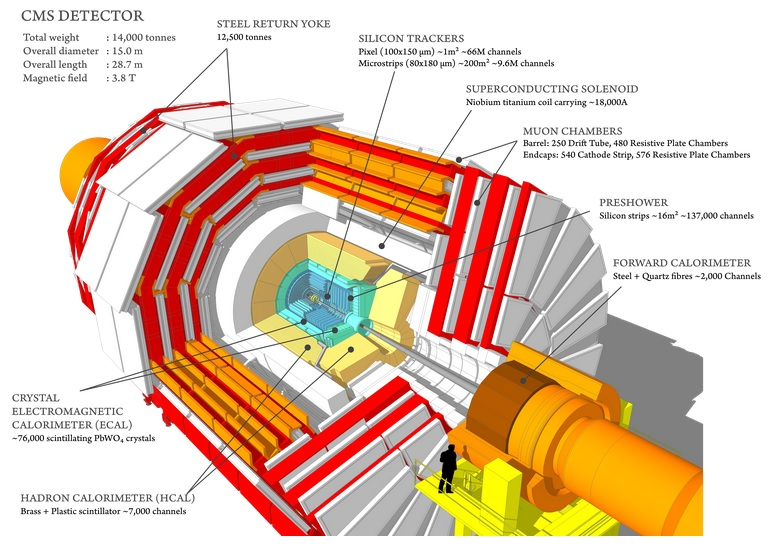
\includegraphics[width=0.8 \textwidth, ext=.png type=jpg]{/home/kpapad/UG_thesis/Thesis/Dissertation/src/figures/cms_detector.jpg}
\caption{A cross-sectional perspective of the CMS detector}
\label{fig:CMS_detector}
\end{figure}

\subsubsection{Coordinate convention at the CMS}
\label{sec:orge8fa37a}
Given the solenoid geometry of the CMS detector, it is more convenient to use a spherical type of coordinates\(\left(r, \phi, \theta \right)\). The origin is located at the collision point and the z axis is parallel to the beam as shown in figure \ref{fig:CMSCoords}. In this system, the momentum of a particle(or any other vector) can be analyzed in a component parallel to the z axis and one component perpendicular to the z axis(Transverse mometnum). Transverse mometnum is defined as follows:
\begin{equation}
|\vec{P_{T}}| = \sqrt{P_{x}^{2} + P_{y}^{2}} = |\vec{P}|\sin{\phi}
\end{equation}
Where \(|\vec{P}| = \sqrt{P_{x}^{2} + P_{y}^{2} + P_{z}^{2}}\). The CMS detector, measures the transverse energy(\href{https://www.lhc-closer.es/taking\_a\_closer\_look\_at\_lhc/0.momentum}{source} ) of particles, and thus it is useful to work with the transverse momentum \(P_{T}\). The azimuth angle  \(\phi \in \left[0, 2\pi\right)\) coordinate is the angle between \(P_{t}\) and x axis and the polar angle  \(\theta \in \left[0, \pi   \right]\) is the angle between the momentum vector and the z axis.

\begin{figure}[ht]
\centering
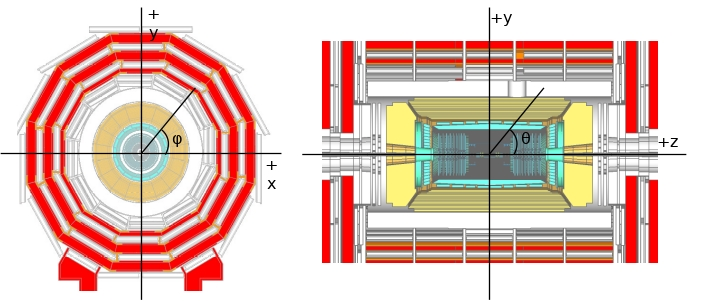
\includegraphics[width=0.7 \textwidth, ext=.png type=jpg]{/home/kpapad/UG_thesis/Thesis/Dissertation/src/figures/cms_coords.jpg}
\caption{CMS coordinates}
\label{fig:CMSCoords}
\end{figure}


Due to the relativistic nature of the phenomena taking place inside LHC, it is more usefull to work with lorentz invariant quantities [V. Chiochia (2010) Accelerators and Particle Detectors from University of Zurich]. Thus, instead of working with the polar angle it is more convenient to introduce the lorentz invariant  \emph{pseudorapidity} \(\eta\in \left [ -\infty, +\infty \right ]\).  Pseudorapidity is defined as:
\begin{equation}
\eta \equiv -\ln{\left [ \tan\left (\frac{\theta}{2} \right ) \right]  }
\end{equation}

The cartesian\(p_{x}\text{, } p_{y}\text{, }p_{z}\) momentum components are related to the \(P_{T}\text{, }\eta\text{, }\phi\)  components by the following transformation relations:
\begin{equation}
\begin{matrix}
p_{x} = P_{T}\cos{\phi} \\
p_{y} = P_{T}\sin{\phi} \\
p_{z} = P_{T}\sinh{\eta}\\
|\vec{P}| = P_{T}\cosh{\eta} 
\end{matrix}
\end{equation}

\subsubsection{Silicon Tracker}
\label{sec:orga7d0d18}
The Silicon tracker measures the positions of charged particles at a number of points, thus it is able to record their trajectory. Given the radius of curvature of the particle's track(due to the 4T magnetic field of the super conducting solenoid), the tracker provides sufficient information, to reconstruct the momentum of the particle. More over, the geometrical location of the trajectory gives direct information regarding the position of the particle. Therefore, the silicon tracker measurements  provide  information regarding the \(P_{T}\text{, } \eta\text{ and }\phi\) of the particles that it detects.

\begin{figure}[ht]
\centering
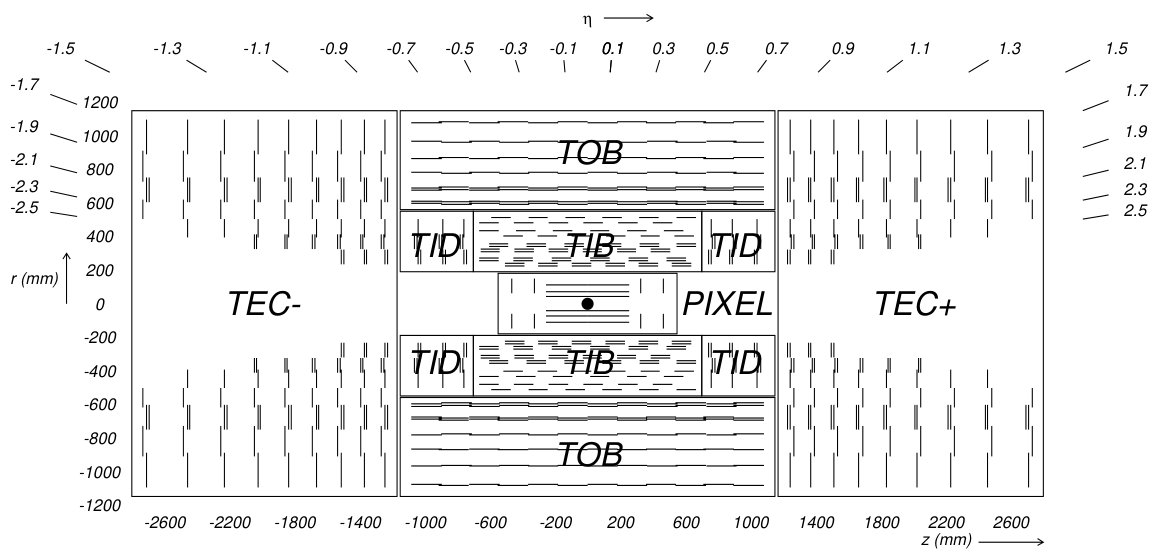
\includegraphics[width=0.9 \textwidth, ext=.png type=jpg]{/home/kpapad/UG_thesis/Thesis/Dissertation/src/figures/cms_tracker.jpg }
\caption{Schemtic illustration of a crossection of the CMS Tracker }
\label{fig:si_tracker}
\end{figure}


A schematic representation of the Sillicon Tracker's corss section, can be viewed on figure \ref{fig:si_tracker}. The tracker consists of a silicon pixel detector and a silicon strip detector. The silicon pixel detector is composed of two sub-detectors. Namely, the barrel which consists of three layers covering the region \(|\eta| < 2.2\) and at \(r = 4.4\text{, }7.3\text{ and }10,2\text{cm}\). The end caps, are two discs of pixel modues, located one on each side, that complete the design of the silicon pixel detector. The pixel detector improrves the trajectory and position measurements, by providing two-dimensional measurements of the charged particles' hit positions. (\href{https://cds.cern.ch/record/1129810}{source}).

The silicon strip detector, covers the radial region \(r \in \left[ 20, 116 \right]\text{cm}\). and  is comprised of four inner barrel (TIB) layers and two inner endcaps (TID). The TIBs are assembled in shells and each TID consists of three small discs. The outer barrel (TOB) encompasses both TIB and TID and contains six concentric layers. The tracker is closed off on either end by two endcaps (TEC). Measurements at the silicon strip detector give information regarding the path of each particle allows the distinction of separate particle trajectories.
